\documentclass[tikz,border=1mm,10pt]{standalone}
%\usepackage[dvipsnames]{xcolor}
\usepackage{pgfplots}
\pgfplotsset{compat=1.5.1}
\usetikzlibrary{arrows}
\usetikzlibrary{patterns}

\begin{document}


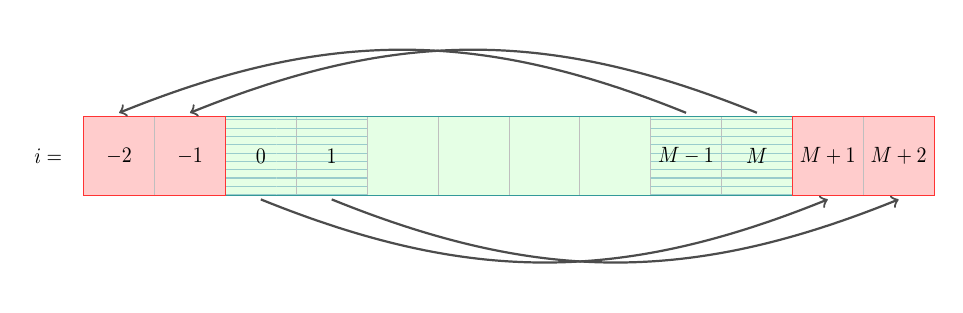
\begin{tikzpicture}[xscale=.9,yscale=1,samples=400, transform shape,every node/.style={scale=.8}]
	%===============
	%	Sequential
	%===============
	
	
	%real Grid
	\filldraw[fill=green!10,draw=teal!80, line width=.15mm] (0, 0) rectangle (8, 1);
	\draw[step=1cm,lightgray,very thin] (0, 0) grid (8,1);
	\draw[draw=teal!80, line width=.15mm] (0, 0) rectangle (8, 1);

	% pattern for real cells
	\fill[pattern=horizontal lines, pattern color=teal!40]  (0,0) rectangle (2, 1);	
	\fill[pattern=horizontal lines, pattern color=teal!40]  (6,0) rectangle (8, 1);	
		
	% Ghost cells left	
	\filldraw[fill=red!20,draw=red!80, line width=.15mm] (-2, 0) rectangle (0, 1);
	\draw[step=1cm,lightgray,very thin] (-2, 0) grid (0,1);
	\draw[draw=red!80, line width=.15mm] (-2, 0) rectangle (0, 1);
	
	%Ghost cells right
	\filldraw[fill=red!20,draw=red!80, line width=.15mm] (8, 0) rectangle (10, 1);
	\draw[step=1cm,lightgray,very thin] (8, 0) grid (10,1);
	\draw[draw=red!80, line width=.15mm] (8, 0) rectangle (10, 1);	

	% Arrows
	\draw[->, black!70, thick] (7.5, 1.05) to[bend right=20] (-0.5,1.05);
	\draw[->, black!70, thick] (6.5, 1.05) to[bend right=20] (-1.5,1.05);
	\draw[->, black!70, thick] (0.5,-0.05) to[bend right=20] (8.5, -0.05);
	\draw[->, black!70, thick] (1.5,-0.05) to[bend right=20] (9.5, -0.05);
	
	% Indices
	\node at (-2.5, 0.5) {$i=$};
	\node at (-1.5, 0.5) {$-2$};
	\node at (-0.5, 0.5) {$-1$};
	\node at (0.5, 0.5)  {$0$};
	\node at (1.5, 0.5)  {$1$};
	
	\node at (6.5, 0.5)  {$M-1$};
	\node at (7.5, 0.5)  {$M$};
	\node at (8.5, 0.5)  {$M+1$};
	\node at (9.5, 0.5)  {$M+2$};

\end{tikzpicture}

\end{document}
